\chapter{Verifica dei collegamenti}
\begin{pycode}[viti]
d = 10 # mm
d1 = 6.2 # mm
#l = 220 # mm 
f_uk = 600 # Mpa
gamma_M1 = 1.05
gamma_M2 = 1.25 # acciao. tabella 4.2 vii ntc
gammaM = 1.5 #connessione in legno 
kmod = 0.9

rho_k1 = 425
rho_k2 = 425

l_ef1 = 80
l_ef2 = 80

V_d = 7704 # N
alpha = 45 # gradi
alpha_fib1 = 90
alpha_fib2 = 45

alpha = np.radians(alpha)


#sistemare per altri angoli!
F_comp = F_traz = V_d * np.cos(alpha)

#################################################

# Verifica A)
A_res = np.pi * d1 **2 / 4
f_ax_rk_vite = 0.9 * A_res * f_uk 
f_ax_rd_vite = f_ax_rk_vite/gamma_M2

# Verifica B)
n_ef = 1 # n**0.9 
f_ax_k_1 = 0.52 * d**-0.5 * l_ef1 **-0.1 * rho_k2**0.8
k_d = min(d/8, 1)

F_ax_rk_1 = (n_ef * f_ax_k_1 * d * l_ef1 * k_d) / (1.2 * np.cos(np.radians(alpha_fib1))**2 + np.sin(np.radians(alpha_fib1))**2)
F_ax_rd_1 = F_ax_rk_1/gammaM * kmod

# Verifica C)
n_ef = 1 # n**0.9 
f_ax_k_2 = 0.52 * d**-0.5 * l_ef2 **-0.1 * rho_k1**0.8
k_d = min(d/8, 1)

F_ax_rk_2 = (n_ef * f_ax_k_2 * d * l_ef2 * k_d) / (1.2 * np.cos(np.radians(alpha_fib2))**2 + np.sin(np.radians(alpha_fib2))**2)
F_ax_rd_2 = F_ax_rk_2/gammaM * kmod

#Verifica D)
N_pl_k = np.pi * d1**2 / 4 * f_uk

c_h = (0.19 + 0.012*d)*rho_k2*((90 + alpha_fib2) / 180)
E_s = 210000
I_s = np.pi * d1**4 / 64
N_ki_k = np.sqrt(c_h * E_s * I_s)

lambda_k = np.sqrt(N_pl_k / N_ki_k)

k = 0.5 * (1 + 0.49*(lambda_k-0.2) + lambda_k**2)
k_c = 1 / (k + np.sqrt(k**2 - lambda_k**2)) if lambda_k > 0.2 else  1

F_ax_rk_buck = N_pl_k * k_c
F_ax_rd_buck = F_ax_rk_buck / gamma_M1
\end{pycode}
%%%%%%%%%%%%%%%%%%%%%
\section{Viti inclinate trave a doppia rastremazione e arcarecci}
\begin{figure}[H]
    \centering
    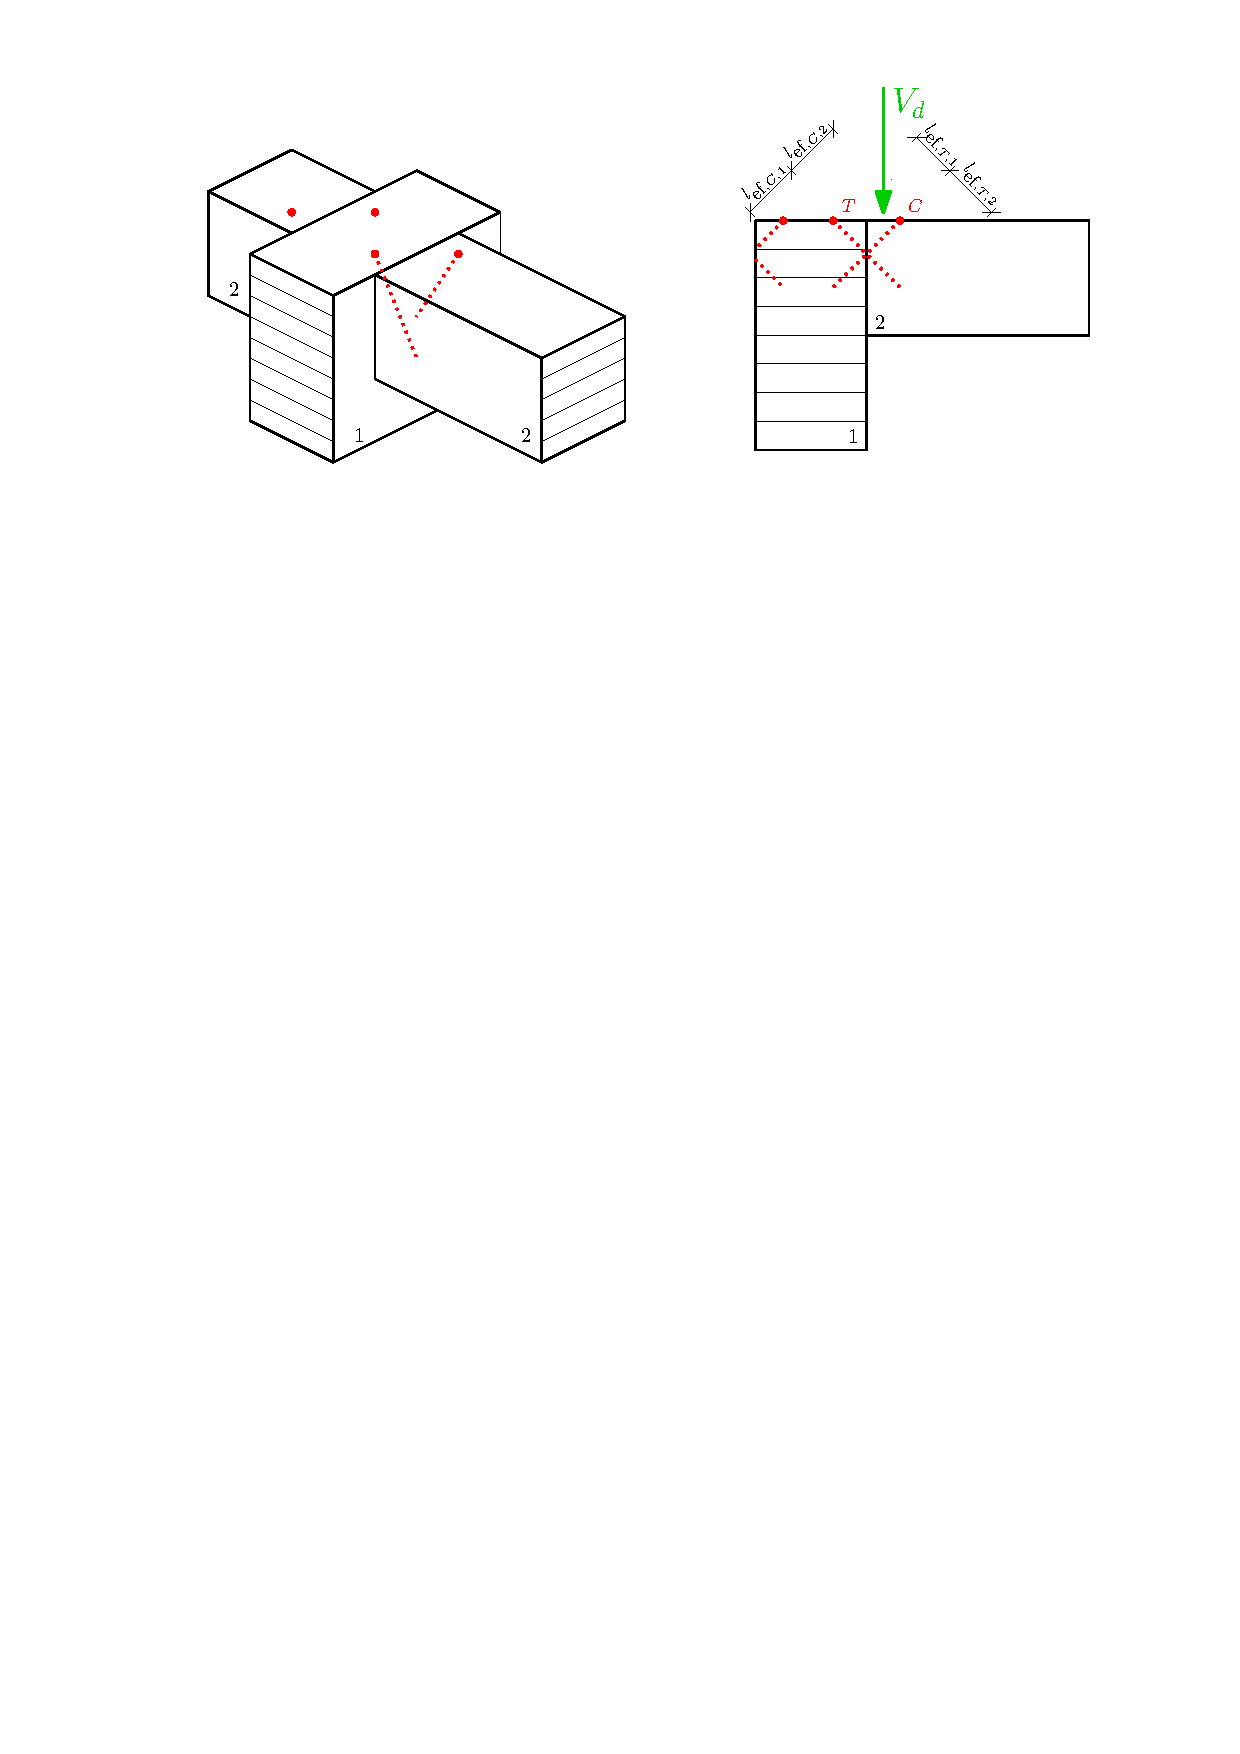
\includegraphics[]{IMG/VitiIncrociate.pdf}
    \caption{Schematizzazione della connessione tramite viti incrociate tra la trave rastremata e gli arcarecci}
    \label{fig:VitiIncrociate}
\end{figure}
\begin{pysub}[viti]
La connessione tra la trave a doppia rastremazione e ciascun arcareccio viene eseguita tramite due viti a tutto filetto.
Entrambe le viti sono sottoggette a puro sforzo assiale ed essendo inclinate ad $\alpha = \SI{45}{\degree}$ gli sforzi valgono 
\begin{equation}
    F_{traz} = F_{comp} = V^{arcareccio} \cos(\alpha) = \SI{!{V_d}}{\newton} \cos\SI{45}{\degree} = \SI{!{round(F_comp,1)}}{\newton} \quad .
\end{equation}
Per la vite sottoposta a sola trazione si tengono conto dei modi di rottura per trazione del materiale acciaio e della rottura per estrazione della vite lato elemento principale $1$ e lato elemento secondario $2$.
Per la vite sottoposta a sola compressione si tiene conto della rottura per estrazione nei due elementi, e della rottura a instabilità per carico di punta a compressione.
Infine si tengono conto delle distanze minime dal bordo e dalle estremità.
\subsection{Resistenze caratteristiche $Rk$}
\paragraph{Rottura acciaio}
\begin{equation}
    F_{ax,Rk}^{acciaio} 
    = 0.9 \, A_{res} \, f_{u,k} 
    = 0.9 \, \dfrac{\pi d_1^2}{4} \, f_{u,k} 
    = \frac{\pi \, (\SI{!{d1}}{\milli\metre})^2}{4} \, \SI{!{f_uk}}{\mega\pascal} 
    = \SI{!{round(f_ax_rk_vite,1)}}{\newton}
\end{equation}

\paragraph{Estrazione elemento 1}
\begin{equation}
    F_{ax,Rk}^{estr. 1} %
    = \frac{f_{ax,k} \cdot d \cdot l_{ef}^i \cdot k_{d} \cdot n_{ef}}%
        {\SI{1.2}{} \cos^2 \alpha_{f-v} + \sin^2 \alpha_{f-v}} %
    = \frac{\SI{!{round(f_ax_k_1,2)}}{} \cdot !{d} \cdot !{l_ef1} \cdot !{k_d} \cdot !{n_ef}}%
        {\SI{1.2}{} \cos^2 !{alpha_fib1} + \sin^2 !{alpha_fib1}} %
    = \SI{!{round(F_ax_rk_1,1)}}{\newton} 
\end{equation}
dove
\[
    \begin{split}
        f_{ax,k} 
        &= \SI{0.52}{} \cdot d^{-0.5} \cdot l_{ef}^{-0.1, \, i} \cdot \rho_k^{0.8, \, i} 
        = \SI{0.52}{} \cdot !{d}^{-0.5} \cdot !{l_ef1}^{-0.1} \cdot !{rho_k2}^{0.8}
        = \SI{!{round(f_ax_k_1,2)}}{\mega\pascal} \\
        %
        k_{d} 
        &= \min \left( \dfrac{d}{8} ; 1 \right)
        =\min \left( \dfrac{!{d}}{8} ; 1 \right) 
        = !{k_d} \\
        %
        \alpha_{f-v}
        &= \SI{!{alpha_fib1}}{\degree} \quad \text{angolo tra la direzione delle fibre e la vite} \\
        %
        n_{ef} 
        &= n^{0.9} 
        = !{n_ef}
    \end{split}
\]

\paragraph{Estrazione elemento 2}
\begin{equation}
    F_{ax,Rk}^{estr. 2} %
    = \frac{f_{ax,k} \cdot d \cdot l_{ef}^i \cdot k_{d} \cdot n_{ef}}%
        {\SI{1.2}{} \cos^2 \alpha_{f-v} + \sin^2 \alpha_{f-v}} %
    = \frac{\SI{!{round(f_ax_k_2,2)}}{} \cdot !{d} \cdot !{l_ef2} \cdot !{k_d} \cdot !{n_ef}}%
        {\SI{1.2}{} \cos^2 !{alpha_fib2} + \sin^2 !{alpha_fib2}} %
    = \SI{!{round(F_ax_rk_2,1)}}{\newton} 
\end{equation}
dove
\[
    \begin{split}
        f_{ax,k} 
        &= \SI{0.52}{} \cdot d^{-0.5} \cdot l_{ef}^{-0.1, \, i} \cdot \rho_k^{0.8, \, i} 
        = \SI{0.52}{} \cdot !{d}^{-0.5} \cdot !{l_ef2}^{-0.1} \cdot !{rho_k1}^{0.8}
        = \SI{!{round(f_ax_k_2,2)}}{\mega\pascal} \\
        %
        k_{d} 
        &= \min \left( \dfrac{d}{8} ; 1 \right)
        =\min \left( \dfrac{!{d}}{8} ; 1 \right) 
        = !{k_d} \\
        %
        \alpha_{f-v}
        &= \SI{!{alpha_fib2}}{\degree} \\
        %
        n_{ef} 
        &= n^{0.9} 
        = !{n_ef}
    \end{split}
\]

\paragraph{Instabilità}
\begin{equation}
    F_{ax,Rk}^{buck} = k_c \cdot N_{pl,k} = \SI{!{round(k_c,3)}}{} \cdot \SI{!{round(N_pl_k,1)}}{\newton} = \SI{!{round(F_ax_rk_buck,1)}}{\newton}
\end{equation}
dove
\[
    \begin{split}
        k_c 
        &= 
        \begin{cases}
            1 & \text{se \quad $ \overline{\lambda}_k \leq 0.2$} \\
            \dfrac{1}{k + \sqrt{k^2 - \overline{\lambda}_k^2 }} & \text{se \quad $\overline{\lambda}_k > 0.2$}
        \end{cases} 
        \quad = \SI{!{round(k_c,3)}}{} \\
        N_{pl,k}
        &= \frac{\pi \, d_1^2}{4} f_{y,k} 
        = \frac{\pi \, (\SI{!{d1}}{\milli\metre})^2}{4} \, \SI{!{f_uk}}{\mega\pascal}
        = \SI{!{round(N_pl_k,1)}}{\newton}\\
    \end{split}
\]
in cui
\[
    \begin{split}
        k 
        &= 0.5 \left[ 1 + 0.49 \left(\overline{\lambda}_k - 0.2 \right) + \overline{\lambda}_k^2 \right]
        = 0.5 \left[ 1 + 0.49 \left(!{round(lambda_k,3)} - 0.2 \right) + !{round(lambda_k,3)}^2 \right] 
        = \SI{!{round(k,4)}}{} \\
        \overline{\lambda}_k
        &= \sqrt{\frac{N_{pl,k}}{N_{ki,k}}}
        = \sqrt{\frac{\SI{!{round(N_pl_k,1)}}{\newton}}{\SI{!{round(N_ki_k,1)}}{\newton}}} 
        = \SI{!{round(lambda_k,3)}}{} \\
        N_{ki,k}
        &= \sqrt{c_h E_s I_s} 
        = \sqrt{\SI{!{round(c_h,2)}}{} \cdot \SI{!{E_s}}{} \cdot \SI{!{round(I_s,3)}}{}}
        = \SI{!{round(N_ki_k,1)}}{\newton}\\
        c_h 
        &= (0.19 + 0.012 \, d) \, \rho_k^i \dfrac{\SI{90}{\degree} + \alpha_{f-v}^i}{\SI{180}{\degree}}
        = (0.19 + 0.012 \, d) \, \SI{!{rho_k2}}{} \dfrac{90 + !{alpha_fib2}}{180} 
        = \SI{!{round(c_h,2)}}{} \\
        & \qquad\text{in cui si è preso il minore tra le due combinazioni di $\alpha_{f-v}$ e $\rho_k$}\\ 
        E_s
        &= \SI{!{E_s}}{\mega\pascal}\\
        I_s
        &= \frac{\pi \, d_1^4}{64}
        = \frac{\pi \, \SI{!{d1}}{}^4}{64}
        = \SI{!{round(I_s,3)}}{\milli\metre\tothe{4}}
    \end{split}
\]

\subsection{Resistenze di progetto $Rd$ e verifica}
\begin{align}
    F_{ax,Rd}^{acciaio} 
    &= \dfrac{F_{ax,Rk}^{acciaio}}{\gamma_{M2}} 
    = \dfrac{\SI{!{round(f_ax_rk_vite,1)}}{\newton}}{!{gamma_M2}} 
    = \SI{!{round(f_ax_rd_vite,1)}}{\newton} \label{eq:viti_a} \\
    %
    F_{ax,Rd}^{estr. 1} 
    &= \dfrac{k_{mod} \cdot F_{ax,Rk}^{estr. 1}}{\gamma_{M}} 
    = \dfrac{!{kmod} \cdot \SI{!{round(F_ax_rk_1,1)}}{\newton}}{!{gammaM}} 
    = \SI{!{round(F_ax_rd_1,1)}}{\newton} \label{eq:viti_b} \\
    F_{ax,Rd}^{estr. 2} 
    %
    &= \dfrac{k_{mod} \cdot F_{ax,Rk}^{estr. 2}}{\gamma_{M}} 
    = \dfrac{!{kmod} \cdot \SI{!{round(F_ax_rk_2,1)}}{\newton}}{!{gammaM}} 
    = \SI{!{round(F_ax_rd_2,1)}}{\newton} \label{eq:viti_c} \\
    %
    F_{ax,Rd}^{buck} 
    &= \dfrac{F_{ax,Rk}^{buck}}{\gamma_{M1}} 
    = \dfrac{\SI{!{round(F_ax_rk_buck,1)}}{\newton}}{!{gamma_M1}} 
    = \SI{!{round(F_ax_rd_buck,1)}}{\newton} \label{eq:viti_d}
\end{align}

Avendo una sola vite per tipologia di sollecitazione $n_{ef} = 1$, quindi le resistenze del singolo connettore corrispondono alle resistenze totali della connessione. 
Per la sollecitazione di trazione si deve avere 
\[
    \min[\text{eqq.} \, (\ref{eq:viti_a}), (\ref{eq:viti_b}), (\ref{eq:viti_c})] = \SI{!{round(min(f_ax_rd_vite,F_ax_rd_1,F_ax_rd_2),1)}}{\newton} > F_{traz} = \SI{!{round(F_traz,1)}}{\newton} ;
\] 
mentre per quella di compressione compressione 
\[
    \min[\text{eqq.} \, (\ref{eq:viti_b}), (\ref{eq:viti_c}), (\ref{eq:viti_d})] = \SI{!{round(min(F_ax_rd_1,F_ax_rd_2,F_ax_rd_buck),1)}}{\newton} > F_{comp} = \SI{!{round(F_comp,1)}}{\newton} .
\]
Le verifiche sono pertanto soddisfatte.

\subsection{Distanze minime e distanze effettive}

\end{pysub}
